\documentclass{article}
\usepackage[T1]{fontenc}
\usepackage{lmodern}
\usepackage{graphicx}
\usepackage{amsmath,amssymb}
\usepackage[a4paper,margin=2cm]{geometry}
\usepackage[absolute,overlay]{textpos}
\setlength{\TPHorizModule}{1mm}
\setlength{\TPVertModule}{1mm}
\usepackage[indonesian]{babel}
\usepackage{hyperref}
\setlength{\emergencystretch}{2em}
% unit: Halaman 3

\begin{document}

% === Halaman 3 (python/native) ===

3

• Tabel substitusi dapat dibentuk secara acak seperti contoh berikut:

• Atau berdasarkan kalimat kunci yang mudah diingat:

 Contoh: di bawah sinar bulan purnama hati resah jadi senang


 Buang duplikasi huruf menjadi: dibawhsnrulpmtejg

 Sambung dengan huruf lain yang belum ada:


 dibawhsnrulpmtejgcfkoqvwxyz

 Tabel substitusi yang dihasilkan:

 Plainteks :  A B C D E F G H I J K L M N O P Q R S T U V W X Y Z

 Cipherteks : D I B A W H S N R U L P M T E J G C F K O V W X Y Z 

Plainteks:

Cipherteks:

% deskripsi: gambar native xref 36
\noindent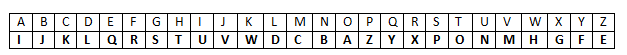
\includegraphics[width=0.85\textwidth]{../../images/python/page_003_img_01.png}

\end{document}
